\documentclass[tikz]{standalone}


% \usepackage[review]{acl}
\usepackage{times}
\usepackage{latexsym}
\usepackage[T1]{fontenc}
\usepackage[utf8]{inputenc}
\usepackage{microtype}
\usepackage{inconsolata}
\usepackage{graphicx}
\usepackage{arydshln}
\usepackage{pifont}


\usepackage{booktabs}
\usepackage{tikz}
\usepackage{pgfplots}
\usepackage{multirow}
\usetikzlibrary{positioning,calc}%
\usetikzlibrary{backgrounds}
\usepackage{color, colortbl}
\usetikzlibrary{decorations.fractals}
\usetikzlibrary{patterns}
\usepackage{booktabs}
\usepackage[dvipsnames]{xcolor}
\usepackage{amsmath}
\usepackage{url}
\usepackage{amssymb}
\usepackage{hyperref}
\usepackage{makecell}
\usepackage[table]{xcolor}

\definecolor{myYellow}{rgb}{0.9,0.9,1}
\definecolor{WindowsBlue}{RGB}{2,152,219}
\definecolor{battleshipgrey}{rgb}{0.3, 0.3, 0.3}
\definecolor{brilliantrose}{rgb}{1.0, 0.33, 0.64}
\definecolor{americanrose}{rgb}{1.0, 0.01, 0.24}
\definecolor{jweigreen}{rgb}{0,0.45,0.24}
\definecolor{bluegray}{rgb}{0.1, 0.1, 0.4}
\definecolor{ao(english)}{rgb}{0.0, 0.5, 0.0}
\definecolor{blanchedalmond}{rgb}{1.0, 0.92, 0.8}
\definecolor{atomictangerine}{rgb}{1.0, 0.6, 0.4}
\definecolor{chocolate(web)}{rgb}{0.82, 0.41, 0.12}
\definecolor{bananayellow}{rgb}{1.0, 0.88, 0.21}
\definecolor{goldenbrown}{rgb}{0.6, 0.4, 0.08}
\definecolor{aliceblue}{rgb}{0.94, 0.97, 1.0}
\definecolor{beige}{rgb}{0.96, 0.96, 0.86}
\definecolor{babyblue}{rgb}{0.54, 0.81, 0.94}
\definecolor{camel}{rgb}{0.76, 0.6, 0.42}
\definecolor{cinnamon}{rgb}{0.82, 0.41, 0.12}



\begin{document}



% \begin{tikzpicture}

% \def\encw{4.0em}
% \def\ench{5em}


% \def\backw{12em}

% \def\nodew{4em}

% \def\adpw{3.0em}
% \def\adph{1.0em}


% \def\hiddenfsep{0.6em}
% \def\hiddensep{0.2em}

% \def\epw{1.5em}
% \def\eph{1.5em}
% \def\sqwh{0.5em}
% \def\pwsep{0.1em}

% \tikzstyle{encodernode}=[minimum height=\ench,minimum width=\encw,inner sep=0,fill=gray!10,rounded corners=2pt,font=\footnotesize, font=\small, align=center];

% \tikzstyle{backnode}=[minimum height=\ench*3.2,minimum width=\backw,inner sep=0,rounded corners=2pt,font=\footnotesize, draw=gray, dashed];

% \tikzstyle{adapternode}=[minimum height=\adph,minimum width=\adpw,inner sep=0,fill=gray,rounded corners=2pt,font=\footnotesize,text=white, align=center];



% \tikzstyle{expertnode}=[minimum height=\adph,minimum width=\adpw,inner sep=0,fill=gray,rounded corners=2pt,font=\footnotesize,text=white, align=center];

% \tikzstyle{sqnode}=[minimum height=\sqwh,minimum width=\sqwh,inner sep=0,font=\tiny,text=white, align=center];












% \def\llmw{2.7in}
% \def\llmh{1.8em}
% \tikzstyle{llmnode}=[minimum height=\llmh,minimum width=\llmw,inner sep=0,fill=black!6,rounded corners=3pt, align=center];

% \def\enchsep{0.8em}
% \def\hiddenfsep{1em}

% \def\encw{4em}
% \def\ench{1.5em}
% \tikzstyle{encodernode}=[minimum height=\ench,minimum width=\encw,inner sep=0,fill=gray!10,rounded corners=2pt,font=\footnotesize, font=\small, rotate=90];

% \def\exwh{1.0em}
% \def\gatew{0.4em}
% \tikzstyle{pnode}=[minimum width=\gatew,fill=Maroon!30,rounded corners=1pt,inner sep=0,font=\footnotesize];
% \tikzstyle{gatebg}=[minimum height=\gatew*8,minimum width=\gatew*10,inner sep=0,font=\footnotesize, align=center,fill=black!6,draw];
% \tikzstyle{expnode}=[minimum height=\exwh,minimum width=\exwh,inner sep=0,font=\footnotesize, align=center,fill=Maroon!30];

% \def\csize{8pt}

% \def\MoEw{2.7in}
% \def\MoEh{1.66in}
% \tikzstyle{moenode}=[minimum height=\MoEh,minimum width=\MoEw,inner sep=0,rounded corners=2pt,font=\footnotesize, draw=gray, thick];

% \def\hiddenh{0.3em}
% \def\hiddenw{3.0em}
% \tikzstyle{whispernode}=[minimum height=\hiddenw,minimum width=\hiddenh,inner sep=0pt,fill=teal!30, align=center,rounded corners=1.2pt];
% \tikzstyle{wavlmnode}=[minimum height=\hiddenw,minimum width=\hiddenh,inner sep=0pt,fill=Tan!30, align=center,rounded corners=1.2pt];
% \tikzstyle{wav2vec2node}=[minimum height=\hiddenw,minimum width=\hiddenh,inner sep=0pt,fill=DarkOrchid!30, align=center,rounded corners=1.2pt];

% \def\sqwh{0.8em}
% \tikzstyle{wbgnode}=[minimum height=\sqwh*1.4,minimum width=\sqwh*7.2,inner sep=0,rounded corners=0pt,font=\footnotesize,fill=gray!10, draw, dashed];
% \tikzstyle{sqnode}=[minimum height=\sqwh,minimum width=\sqwh,inner sep=0,font=\tiny, align=center,fill=gray!80];

% \tikzstyle{fusionbg}=[minimum height=\hiddenh*8,minimum width=\hiddenw*1.7,inner sep=0pt, align=center,rounded corners=1.2pt,draw,dashed];
% \tikzstyle{fusionnode}=[minimum height=\hiddenh,minimum width=\hiddenw,inner sep=0pt, align=center,fill=gray!80,rounded corners=1.2pt];

% \tikzstyle{FFNnode}=[minimum height=\hiddenh*3,minimum width=\hiddenw*1.7,inner sep=0pt, align=center,rounded corners=1.2pt,draw,rotate=90];


% \begin{scope}[]

% \node [anchor=north west, llmnode] (llm) at (0,0) {LLM};
% \node [anchor=north west, font=\scriptsize, align=center] (prompt) at ([yshift=-\hiddenfsep*4.2]llm.south west) {Hear the audio clip and transform \\ it into text format. <|AUDIO|>};
% \node [anchor=north east, draw] (audio) at ([yshift=-0.5em]prompt.south east) {\includegraphics[width=2cm]{../Figures/audio.png}};

% \node [anchor=south east, fill=gray,opacity=0.15, minimum height=0.5em,minimum width=3.3em] (promptaudio) at ([xshift=-0.7em, yshift=0.2em]prompt.south east) {};

% \node [anchor=south west, gatebg] (gtbg) at ([xshift=\hiddenfsep*4.0, yshift=-\hiddenfsep*4.0]llm.south west) {};
% \node [anchor=south west, pnode, minimum height=1.3em] (p3) at ([xshift=\hiddenfsep*0.3, yshift=\hiddenfsep*0.8]gtbg.south west) {};
% \node [anchor=south west,pnode,minimum height=1.7em, draw=Maroon] (p2) at ([xshift=\pwsep,yshift=0em]p3.south east) {};
% \node [anchor=south west] (pi) at ([xshift=\pwsep,yshift=0em]p2.south east) {$\ldots$};
% \node [anchor=south west,pnode,minimum height=0.6em] (p1) at ([xshift=\pwsep,yshift=0em]pi.south east) {};

% \node [anchor=north,font=\tiny,gray] (x1) at ([xshift=\hiddenfsep*0.0, yshift=\hiddenfsep*0.1]p3.south) {\textbf{1}};
% \node [anchor=north,font=\tiny,Maroon] (x2) at ([xshift=\hiddenfsep*0.0, yshift=\hiddenfsep*0.1]p2.south) {\textbf{2}};
% \node [anchor=north,font=\tiny,gray] (xn) at ([xshift=\hiddenfsep*0.0, yshift=\hiddenfsep*0.1]p1.south) {$\mathbf{N}$};

% \node [anchor=north east, minimum height=\encw*1.2,minimum width=\ench*4.5,fill=black!6,rounded corners=2pt] (encbg) at ([xshift=-0.0em, yshift=-\hiddenfsep*5.5]llm.south east) {};
% \node [anchor=north, encodernode, draw=teal, thick] (encoder1) at ([xshift=\hiddenfsep*0.3]encbg.west) {Whisper};
% \node [anchor=north, encodernode, draw=Tan, thick] (encoder2) at ([xshift=\enchsep*0.9]encoder1.south) {WavLM};
% \node [anchor=north, encodernode, draw=DarkOrchid, thick] (encoder3) at ([xshift=\enchsep*0.9]encoder2.south) {Wav2Vec2};


% %%%%%%%-routing-probability
% \node [anchor=south, minimum height=\encw*0.4,minimum width=\ench*4.5,fill=black!6,rounded corners=2pt] (expertbg) at ([yshift=\hiddenfsep*1.7]encbg.north) {};
% \node [anchor=west, expnode, fill=Maroon!50] (exp1) at ([xshift=\hiddenfsep*0.2]expertbg.west) {S};
% \node [anchor=west, expnode] (exp2) at ([xshift=\hiddenfsep*0.3]exp1.east) {1};
% \node [anchor=west, expnode] (exp3) at ([xshift=\hiddenfsep*0.3]exp2.east) {2};
% \node [anchor=west, expnode] (expi) at ([xshift=\hiddenfsep*0.3]exp3.east) {$\ldots$};
% \node [anchor=west, expnode] (exp4) at ([xshift=\hiddenfsep*0.3]expi.east) {$N$};

% \node [anchor=east,font=\scriptsize,text=gray] (explabel) at ([xshift=-\hiddenfsep*0.0]expertbg.west) {\textbf{Experts}};
% \node [anchor=north east,font=\scriptsize,text=gray] (routerlabel) at ([yshift=-\hiddenfsep*0.3]explabel.south east) {\textbf{Router}};

% \node[anchor=south, draw, thick, inner sep=0pt, circle, minimum size=\csize] (c1) at ([xshift=\hiddenfsep*0, yshift=\hiddenfsep*0.5]expertbg.north) {};
% \draw[-,thick] (c1.north)--(c1.south);
% \draw[-,thick] (c1.west)--(c1.east);


% %%%%%%%%-expert-legend
% \node [anchor=south west, expnode, fill=Maroon!50] (sexplegend) at ([xshift=\hiddenfsep*0.0,yshift=\hiddenfsep*0.3]llm.north west) {S};
% \node [anchor=west, font=\footnotesize] (sexplegendtag) at ([xshift=\hiddenfsep*0.1,yshift=\hiddenfsep*0.0]sexplegend.east) {Shared Expert};
% \node [anchor=west, expnode] (explegend) at ([xshift=\hiddenfsep*0.1]sexplegendtag.east) {};
% \node [anchor=west, font=\footnotesize] (explegendtag) at ([xshift=\hiddenfsep*0.1,yshift=\hiddenfsep*0.0]explegend.east) {Routed Expert};


% %%%%%%%%-expert-fusion-baskground
% \node [anchor=south west, moenode] (moeback) at ([xshift=\hiddenfsep*1.0, yshift=0em]encbg.south east) {};
% \node [anchor=south west, font=\footnotesize, text=gray] (moelabel) at ([xshift=\hiddenfsep*0, yshift=\hiddenfsep*0.0]moeback.north west) {\textbf{Expert} $\mathbf{i}$};

% \node [anchor=south west, whispernode,fill=teal] (whis1) at ([xshift=\hiddenfsep*1.2, yshift=\hiddenfsep*0.5]moeback.south west) {};
% \node [anchor=south west, whispernode] (whis2) at ([xshift=\hiddensep*1.6]whis1.south east) {};
% \node [anchor=south west, whispernode] (whis3) at ([xshift=\hiddensep*1.6]whis2.south east) {};
% \node [anchor=west, align=center] (whisi) at ([xshift=0em]whis3.east) {$\ldots$};
% \node [anchor=west, whispernode] (whis4) at ([xshift=\hiddensep*1.6]whisi.east) {};

% \node [anchor=south west, wavlmnode,fill=Tan] (wavlm1) at ([xshift=\hiddenfsep*2.4, yshift=0em]whis4.south east) {};
% \node [anchor=south west, wavlmnode] (wavlm2) at ([xshift=\hiddensep*1.6]wavlm1.south east) {};
% \node [anchor=south west, wavlmnode] (wavlm3) at ([xshift=\hiddensep*1.6]wavlm2.south east) {};
% \node [anchor=west, align=center] (wavlmi) at ([xshift=0em]wavlm3.east) {$\ldots$};
% \node [anchor=west, wavlmnode] (wavlm4) at ([xshift=\hiddensep*1.6]wavlmi.east) {};

% \node [anchor=south west, wav2vec2node,fill=DarkOrchid] (wav2vec1) at ([xshift=\hiddenfsep*2.4, yshift=0em]wavlm4.south east) {};
% \node [anchor=south west, wav2vec2node] (wav2vec2) at ([xshift=\hiddensep*1.6]wav2vec1.south east) {};
% \node [anchor=south west, wav2vec2node] (wav2vec3) at ([xshift=\hiddensep*1.6]wav2vec2.south east) {};
% \node [anchor=west, align=center] (wav2veci) at ([xshift=0em]wav2vec3.east) {$\ldots$};
% \node [anchor=west, wav2vec2node] (wav2vec4) at ([xshift=\hiddensep*1.6]wav2veci.east) {};

% %%%%%%%%%-fusion weight matrix
% \node [anchor=south west, wbgnode,fill=black!0, minimum height=\sqwh*5.7,minimum width=\sqwh*8.0, draw=none] (wbgall) at ([xshift=0em, yshift=\hiddenfsep*1.6]whis1.north west) {};
% \node [anchor=west, wbgnode,fill=teal!30, minimum height=\sqwh*5.7,minimum width=\sqwh*2.6, draw=none] (wbgenc1) at ([xshift=0em, yshift=0em]wbgall.west) {};
% \node [anchor=west, wbgnode,fill=Tan!30, minimum height=\sqwh*5.7,minimum width=\sqwh*2.6, draw=none] (wbgenc2) at ([xshift=0em, yshift=0em]wbgenc1.east) {};
% \node [anchor=west, wbgnode,fill=DarkOrchid!30, minimum height=\sqwh*5.7,minimum width=\sqwh*2.6, draw=none] (wbgenc3) at ([xshift=0em, yshift=0em]wbgenc2.east) {};
% \node [anchor=south,teal,font=\tiny] (encl1) at ([xshift=0em, yshift=-\sqwh*0.3]wbgenc1.north) {$L_1 - 1$};
% \node [anchor=south,Tan,font=\tiny] (encl2) at ([xshift=0em, yshift=-\sqwh*0.3]wbgenc2.north) {$L_2 - 1$};
% \node [anchor=south,DarkOrchid,font=\tiny] (encl3) at ([xshift=0em, yshift=-\sqwh*0.3]wbgenc3.north) {$L_3 - 1$};

% \node [anchor=south, wbgnode] (wbg1) at ([xshift=0em, yshift=\hiddenfsep*0.2]wbgall.south) {};
% \node [anchor=south west, wbgnode] (wbg2) at ([xshift=0em, yshift=\hiddenfsep*0.3]wbg1.north west) {};
% \node [anchor=south west, wbgnode] (wbg3) at ([xshift=0em, yshift=\hiddenfsep*0.3]wbg2.north west) {};
% \node [anchor=south, font=\scriptsize] (labelfw) at ([xshift=\hiddenfsep*0, yshift=\hiddenfsep*0.8]wbg3.north) {Fusion weight matrix};

% \draw [decorate,decoration={brace,amplitude=3pt}, draw] ([xshift=-0.1em]wbg1.south west) -- ([xshift=-0.1em]wbg3.north west) node [midway, xshift=-0.6em, yshift=-0.5em, above, font=\tiny] (fusek) {$k$};

% \node [anchor=west, sqnode] (fw11) at ([xshift=0.2em, yshift=0em]wbg1.west) {.3};
% \node [anchor=west, sqnode] (fw12) at ([xshift=0.05em, yshift=0em]fw11.east) {.1};
% \node [anchor=west, sqnode] (fw13) at ([xshift=0.05em, yshift=0em]fw12.east) {.0};
% \node [anchor=west] (fwi1) at ([xshift=0.0em, yshift=0em]fw13.east) {$\ldots$};
% \node [anchor=west, sqnode] (fw14) at ([xshift=0.05em, yshift=-0em]fwi1.east) {.8};

% \node [anchor=west, sqnode] (fw21) at ([xshift=0.2em, yshift=0em]wbg2.west) {.7};
% \node [anchor=west, sqnode] (fw22) at ([xshift=0.05em, yshift=0em]fw21.east) {.3};
% \node [anchor=west, sqnode] (fw23) at ([xshift=0.05em, yshift=0em]fw22.east) {.1};
% \node [anchor=west] (fwi2) at ([xshift=0.0em, yshift=0em]fw23.east) {$\ldots$};
% \node [anchor=west, sqnode] (fw24) at ([xshift=0.05em, yshift=-0em]fwi2.east) {.2};

% \node [anchor=west, sqnode] (fw31) at ([xshift=0.2em, yshift=0em]wbg3.west) {.0};
% \node [anchor=west, sqnode] (fw32) at ([xshift=0.05em, yshift=0em]fw31.east) {.6};
% \node [anchor=west, sqnode] (fw33) at ([xshift=0.05em, yshift=0em]fw32.east) {.9};
% \node [anchor=west] (fwi3) at ([xshift=0.0em, yshift=0em]fw33.east) {$\ldots$};
% \node [anchor=west, sqnode] (fw34) at ([xshift=0.05em, yshift=-0em]fwi3.east) {.6};

% \draw [decorate,decoration={brace,amplitude=2pt}, draw=teal] ([yshift=0.05em]whis2.north west) -- ([yshift=0.05em]whis4.north east) node [midway, xshift=0.0em, above] (dec1) {};
% \draw [decorate,decoration={brace,amplitude=2pt}, draw=Tan] ([yshift=0.05em]wavlm2.north west) -- ([yshift=0.05em]wavlm4.north east) node [midway, xshift=0.0em, above] (dec2) {};
% \draw [decorate,decoration={brace,amplitude=2pt}, draw=DarkOrchid] ([yshift=0.05em]wav2vec2.north west) -- ([yshift=0.05em]wav2vec4.north east) node [midway, xshift=0.0em, above] (dec3) {};


% \node [anchor=south west, fusionbg] (lastbg1) at ([xshift=\hiddenfsep*1.8, yshift=0em]wbg1.south east) {};
% \node [anchor=south, fusionbg] (lastbg2) at ([xshift=0em, yshift=\hiddenfsep*0.7]lastbg1.north) {};

% \node [anchor=south, fusionnode] (lfusion1) at ([xshift=\hiddenfsep*0, yshift=0.2em]lastbg1.south) {};
% \node [anchor=south, fusionnode] (lfusion2) at ([xshift=\hiddenfsep*0, yshift=\hiddenfsep*0.1]lfusion1.north) {};
% \node [anchor=south, fusionnode] (lfusion3) at ([xshift=\hiddenfsep*0, yshift=\hiddenfsep*0.1]lfusion2.north) {};
% \node [anchor=south, font=\tiny] (labelf1) at ([xshift=\hiddenfsep*0, yshift=\hiddenfsep*0.0]lfusion3.north) {Fused Hidden States};

% \node [anchor=south, fusionnode,fill=DarkOrchid] (wav2vecf1) at ([xshift=\hiddenfsep*0, yshift=0.2em]lastbg2.south) {};
% \node [anchor=south, fusionnode,fill=Tan] (wavlmf1) at ([xshift=\hiddenfsep*0, yshift=\hiddenfsep*0.1]wav2vecf1.north) {};
% \node [anchor=south, fusionnode,fill=teal] (whisf1) at ([xshift=\hiddenfsep*0, yshift=\hiddenfsep*0.1]wavlmf1.north) {};
% \node [anchor=south, font=\tiny] (labelf2) at ([xshift=\hiddenfsep*0, yshift=\hiddenfsep*0.0]whisf1.north) {Last Hidden States};

% \node [anchor=north west, FFNnode] (ffn) at ([xshift=\hiddenfsep*1.8, yshift=0.0em]lastbg1.south east) {FFN};

% \node [anchor=west, whispernode, fill=gray!80] (finalfusion) at ([xshift=\hiddenfsep*1.5, yshift=0.0em]ffn.south) {};

% %%%%%%%-line in left part
% \draw[->,thick,gray] ([xshift=0.2em, yshift=-0.0em]audio.east) -- ([xshift=\hiddenfsep*2.4, yshift=-0.0em]audio.east);
% \draw[->,thick,gray] ([xshift=\hiddenfsep*1.2, yshift=-0.0em]prompt.north west) -- ([xshift=\hiddenfsep*1.2, yshift=-0.1em]llm.south west);

% \draw[->,thick,gray] ([xshift=0.0em, yshift=-0.0em]promptaudio.south) -- ([xshift=0.0em, yshift=-\hiddenfsep*0.6]promptaudio.south);

% \draw[->,thick,gray] ([xshift=\hiddenfsep*1.2, yshift=0.0em]llm.north west) .. controls +(east:0.02em) and +(north:\llmh*1.5) .. ([xshift=\hiddenfsep*2.5, yshift=0.0em]llm.south west) .. controls +(south:1.5em) and +(west:0.8em) .. ([xshift=-0.2em]gtbg.west);
% \draw[->,thick,gray] ([xshift=0.1em, yshift=0.0em]gtbg.east) .. controls +(east:0.8em) and +(west:0.8em) .. ([xshift=0.1em, yshift=0.0em]routerlabel.west);




% %%%%%%%-routing-line
% % \draw[->,thick] ([xshift=0.0em, yshift=0.0em]encbg.north) .. controls +(north:1.5em) and +(south:1.5em) .. ([xshift=0.0em, yshift=-0.1em]exp1.south);
% % \draw[->,thick, Maroon,dashed] ([xshift=0.0em, yshift=0.0em]encbg.north) .. controls +(north:1.0em) and +(south:1.0em) .. ([xshift=0.0em, yshift=-0.1em]exp2.south);
% % \draw[->,thick, Maroon] ([xshift=0.0em, yshift=0.0em]encbg.north) .. controls +(north:0.2em) and +(south:0.2em) .. ([xshift=0.0em, yshift=-0.1em]exp3.south);
% % \draw[->,thick, Maroon,dashed] ([xshift=0.0em, yshift=0.0em]encbg.north) .. controls +(north:1.5em) and +(south:1.5em) .. ([xshift=0.0em, yshift=-0.1em]exp4.south);

% % \draw[->,thick] ([xshift=0.0em, yshift=0.0em]exp1.north) .. controls +(north:1.3em) and +(south:0.8em) .. ([xshift=0.0em, yshift=-0.0em]c1.south);
% % \draw[->,thick, Maroon] ([xshift=0.0em, yshift=0.0em]exp3.north) .. controls +(north:0.2em) and +(south:0.2em) .. ([xshift=0.0em, yshift=-0.0em]c1.south);

% % \draw[->,thick, gray] ([xshift=0.0em, yshift=0.0em]encbg.north) -- ([xshift=0.0em, yshift=\hiddenfsep*0.5]encbg.north) -- ([xshift=0.0em, yshift=-\hiddenfsep*1.25]exp2.south) -- ([xshift=0.0em, yshift=-0.1em]exp2.south);
% % \draw[->,thick, gray] ([xshift=0.0em, yshift=0.0em]encbg.north) -- ([xshift=0.0em, yshift=\hiddenfsep*0.5]encbg.north) -- ([xshift=0.0em, yshift=-\hiddenfsep*1.25]expi.south) -- ([xshift=0.0em, yshift=-0.1em]expi.south);
% \draw[->,thick, gray, dashed] ([xshift=0.0em, yshift=0.0em]encbg.north) -- ([xshift=0.0em, yshift=\hiddenfsep*0.5]encbg.north) -- ([xshift=0.0em, yshift=-\hiddenfsep*0.8]exp2.south) -- ([xshift=0.0em, yshift=-0.1em]exp2.south);
% \draw[->,thick, gray, dashed] ([xshift=0.0em, yshift=0.0em]encbg.north) -- ([xshift=0.0em, yshift=\hiddenfsep*0.5]encbg.north) -- ([xshift=0.0em, yshift=-\hiddenfsep*0.8]expi.south) -- ([xshift=0.0em, yshift=-0.1em]expi.south);
% \draw[->,thick, gray, dashed] ([xshift=0.0em, yshift=0.0em]encbg.north) -- ([xshift=0.0em, yshift=\hiddenfsep*0.5]encbg.north) -- ([xshift=0.0em, yshift=-\hiddenfsep*1.45]exp4.south) -- ([xshift=0.0em, yshift=-0.1em]exp4.south);
% \draw[->,thick, gray] ([xshift=0.0em, yshift=0.0em]encbg.north) -- ([xshift=0.0em, yshift=\hiddenfsep*0.5]encbg.north) -- ([xshift=0.0em, yshift=-\hiddenfsep*1.45]exp1.south) -- ([xshift=0.0em, yshift=-0.1em]exp1.south);
% \draw[->,thick, gray] ([xshift=0.0em, yshift=0.0em]encbg.north) -- ([xshift=0.0em, yshift=-0.1em]exp3.south);

% \draw[->,thick, gray] ([xshift=0.0em, yshift=0.0em]exp1.north) -- ([xshift=0.0em, yshift=\hiddenfsep*1.20]exp1.north) -- ([xshift=-0.1em, yshift=-0.0em]c1.west);
% \draw[->,thick, gray, dashed] ([xshift=0.0em, yshift=0.0em]exp2.north) -- ([xshift=0.0em, yshift=\hiddenfsep*0.3]exp2.north) -- ([xshift=-0.1em, yshift=-0.1em]c1.south west);
% \draw[->,thick, gray] ([xshift=0.0em, yshift=0.0em]exp3.north) -- ([xshift=0.0em, yshift=-0.1em]c1.south);
% \draw[->,thick, gray, dashed] ([xshift=0.0em, yshift=0.0em]expi.north) -- ([xshift=0.0em, yshift=\hiddenfsep*0.3]expi.north) -- ([xshift=0.1em, yshift=-0.1em]c1.south east);
% \draw[->,thick, gray, dashed] ([xshift=0.0em, yshift=0.0em]exp4.north) -- ([xshift=0.0em, yshift=\hiddenfsep*1.20]exp4.north) -- ([xshift=0.1em, yshift=-0.0em]c1.east);



% \draw[->,thick, gray] ([xshift=0.1em, yshift=0.0em]exp4.east) .. controls +(east:0.8em) and +(west:0.8em) .. ([xshift=-0.1em, yshift=-0.0em]moeback.west);

% \draw[->,thick] ([xshift=0.0em, yshift=0.0em]c1.north) -- ([xshift=0.0em, yshift=\hiddenfsep*0.65]c1.north);
% \draw[->,thick, dotted] ([xshift=\hiddenfsep*6.5, yshift=0.0em]llm.north) .. controls +(east:0.02em) and +(north:\llmh*0.9) .. ([xshift=\hiddenfsep*7.0, yshift=\llmh*0.5]llm.south) .. controls +(south:\llmh*1.1) and +(east:0.0em) .. ([xshift=\hiddenfsep*7.5, yshift=0.0em]llm.south);
% \draw[->,thick, dotted] ([xshift=\hiddenfsep*7.5, yshift=0.0em]llm.north) .. controls +(east:0.02em) and +(north:\llmh*0.9) .. ([xshift=\hiddenfsep*8.0, yshift=\llmh*0.5]llm.south) .. controls +(south:\llmh*1.1) and +(east:0.0em) .. ([xshift=\hiddenfsep*8.5, yshift=0.0em]llm.south);
% \draw[->,thick, dotted] ([xshift=\hiddenfsep*8.5, yshift=0.0em]llm.north) .. controls +(east:0.02em) and +(north:\llmh*0.9) .. ([xshift=\hiddenfsep*9.0, yshift=\llmh*0.5]llm.south) .. controls +(south:\llmh*1.1) and +(east:0.0em) .. ([xshift=\hiddenfsep*9.5, yshift=0.0em]llm.south);

% % \draw[->,thick, Gray!65] ([xshift=0.1em, yshift=-0.0em]whisbg.east) .. controls +(east:1.5em) and +(west:1.5em) .. ([xshift=0em]fwbg1.west);

% %%%%%%%%-expert-line
% % \draw[->,thick, teal] ([xshift=0em, yshift=0.1em]dec1.south) .. controls +(north:1.0em) and +(south:1.0em) .. ([xshift=\hiddenfsep*1.5, yshift=-0.1em]wbg1.south);
% % \draw[->,thick, Tan] ([xshift=0em, yshift=0.1em]dec2.south) .. controls +(north:1.2em) and +(south:1.7em) .. ([xshift=\hiddenfsep*1.5, yshift=-0.1em]wbg1.south);
% % \draw[->,thick, DarkOrchid] ([xshift=0em, yshift=0.1em]dec3.south) .. controls +(north:1.5em) and +(south:1.3em) .. ([xshift=\hiddenfsep*1.5, yshift=-0.1em]wbg1.south);

% % \draw[->,thick, teal] ([xshift=0em, yshift=0.1em]dec1.south) -- ([xshift=0em, yshift=\hiddenfsep*1.5]dec1.south);
% \draw[->,thick, teal] ([xshift=0em, yshift=0.1em]dec1.south) -- ([xshift=0em, yshift=\hiddenfsep*0.8]dec1.south) -- ([xshift=-\hiddenfsep*1.3, yshift=\hiddenfsep*0.8]dec1.south) -- ([xshift=-\hiddenfsep*1.3, yshift=\hiddenfsep*1.5]dec1.south);
% \draw[->,thick, Tan] ([xshift=0em, yshift=0.1em]dec2.south) -- ([xshift=0em, yshift=\hiddenfsep*0.6]dec2.south) -- ([xshift=-\hiddenfsep*5.7, yshift=\hiddenfsep*0.6]dec2.south) -- ([xshift=-\hiddenfsep*5.7, yshift=\hiddenfsep*1.5]dec2.south);
% \draw[->,thick, DarkOrchid] ([xshift=0em, yshift=0.1em]dec3.south) -- ([xshift=0em, yshift=\hiddenfsep*1.0]dec3.south) -- ([xshift=-\hiddenfsep*10.3, yshift=\hiddenfsep*1.0]dec3.south) -- ([xshift=-\hiddenfsep*10.3, yshift=\hiddenfsep*1.5]dec3.south);

% % \draw[->,thick,gray] ([xshift=0em, yshift=0.0em]wbg1.east) .. controls +(east:0.8em) and +(west:0.8em) .. ([xshift=0em, yshift=-0.0em]lastbg1.west);
% % \draw[->,thick,gray] ([xshift=0em, yshift=0.0em]wbg2.east) .. controls +(east:0.8em) and +(west:0.8em) .. ([xshift=0em, yshift=-0.0em]lastbg1.west);
% % \draw[->,thick,gray] ([xshift=0em, yshift=0.0em]wbg3.east) .. controls +(east:0.8em) and +(west:0.8em) .. ([xshift=0em, yshift=-0.0em]lastbg1.west);
% \draw[->,thick,gray] ([xshift=-1.5em, yshift=0.0em]lastbg1.west) -- ([xshift=0em, yshift=-0.0em]lastbg1.west);

% \draw[->,thick] ([xshift=0.0em, yshift=-0.0em]lastbg1.east) -- ([xshift=\hiddenfsep*1.8, yshift=-0.0em]lastbg1.east);
% \draw[->,thick] ([xshift=0.0em, yshift=-0.0em]lastbg2.east) -- ([xshift=\hiddenfsep*1.8, yshift=-0.0em]lastbg2.east);

% \draw[->,thick] ([xshift=0.0em, yshift=-0.0em]ffn.south) -- ([xshift=\hiddenfsep*0, yshift=-0.0em]finalfusion.west);

% \end{scope}


% \end{tikzpicture}















% \begin{tikzpicture}

% \def\xsep{2.2em}

% %%%%%%%%%%%%%%%%%-ASR
% \begin{scope}[xshift=0em]
% \begin{axis}[
% at={(0em,0em)},
% width=3.7cm, height=2.8cm,
% xtick=data,
% symbolic x coords={Shallow, Middle, Deep},
% ytick={0.32,0.33,...,0.35},
% xlabel style={align=center,font=\scriptsize,xshift=2.2em},
% ylabel style={font=\scriptsize,yshift=-0.6em},
% x tick label style={opacity=0},
% y tick label style={font=\tiny,/pgf/number format/.cd,fixed,precision=2},
% xmajorgrids=true,
% ymajorgrids=true,
% xtick pos=bottom,
% ytick pos=left,
% major tick length=2pt,
% title={Whisper},
% title style={anchor=center, font=\scriptsize,yshift=0.2em},
% major grid style={gray!30},
% axis on top,
% tick align=outside,
% enlarge x limits=0.2, 
% ymin=0.32, ymax=0.354]

% \addplot[teal, thick, mark=*, mark size=1pt] coordinates {(Shallow, 0.32451508) (Middle, 0.32614517) (Deep, 0.32582941)};

% \end{axis}

% \node [anchor=north west,font=\scriptsize, purple!80!black] (label) at (-0.2em,3em) {\textbf{ASR-clean}};

% \begin{axis}[
% at={(2.12cm,0em)},
% width=3.7cm, height=2.8cm,
% xtick=data,
% symbolic x coords={Shallow, Middle, Deep},
% xlabel style={align=center,font=\scriptsize,xshift=2.2em},
% y tick style={opacity=0},
% x tick label style={opacity=0},
% y tick label style={opacity=0},
% xmajorgrids=true,
% ymajorgrids=true,
% xtick pos=bottom,
% ytick pos=left,
% major tick length=2pt,
% title={WavLM},
% title style={anchor=center, font=\scriptsize,yshift=0.2em},
% major grid style={gray!30},
% axis on top,
% tick align=outside,
% enlarge x limits=0.2, 
% ymin=0.32, ymax=0.354]

% \addplot[orange, thick, mark=*, mark size=1pt] coordinates {(Shallow, 0.33348093) (Middle, 0.33358926) (Deep, 0.34391801)};

% \end{axis}

% \begin{axis}[
% at={(4.24cm,0em)},
% width=3.7cm, height=2.8cm,
% xtick=data,
% symbolic x coords={Shallow, Middle, Deep},
% xlabel style={align=center,font=\scriptsize,xshift=2.2em},
% y tick style={opacity=0},
% x tick label style={opacity=0},
% y tick label style={opacity=0},
% xmajorgrids=true,
% ymajorgrids=true,
% xtick pos=bottom,
% ytick pos=left,
% major tick length=2pt,
% title={Wav2Vec2},
% title style={anchor=center, font=\scriptsize,yshift=0.2em},
% major grid style={gray!30},
% axis on top,
% tick align=outside,
% enlarge x limits=0.2, 
% ymin=0.32, ymax=0.354]

% \addplot[violet, thick, mark=*, mark size=1pt] coordinates {(Shallow, 0.32771354) (Middle, 0.3342245) (Deep, 0.3505841)};

% \end{axis}
% \end{scope}



% %%%%%%%%%%%%%%%%%-ASR-noisy
% \begin{scope}[xshift=0em,yshift=-3.6em]
% \begin{axis}[
% at={(0em,0em)},
% width=3.7cm, height=2.8cm,
% xtick=data,
% symbolic x coords={Shallow, Middle, Deep},
% ytick={0.32,0.33,...,0.35},
% ylabel={\textbf{Weight}},
% xlabel style={align=center,font=\scriptsize,xshift=2.2em},
% ylabel style={font=\scriptsize,yshift=-0.6em,xshift=-1.8em},
% x tick label style={opacity=0},
% y tick label style={font=\tiny,/pgf/number format/.cd,fixed,precision=2},
% xmajorgrids=true,
% ymajorgrids=true,
% xtick pos=bottom,
% ytick pos=left,
% major tick length=2pt,
% major grid style={gray!30},
% axis on top,
% tick align=outside,
% enlarge x limits=0.2, 
% ymin=0.32, ymax=0.354]

% \addplot[teal, thick, mark=*, mark size=1pt] coordinates {(Shallow, 0.32715681) (Middle, 0.3323118) (Deep, 0.34617039)};

% \end{axis}

% \node [anchor=north west,font=\scriptsize, purple!80!black] (label) at (-0.2em,3em) {\textbf{ASR-noisy}};


% \begin{axis}[
% at={(2.12cm,0em)},
% width=3.7cm, height=2.8cm,
% xtick=data,
% symbolic x coords={Shallow, Middle, Deep},
% xlabel style={align=center,font=\scriptsize,xshift=2.2em},
% y tick style={opacity=0},
% x tick label style={opacity=0},
% y tick label style={opacity=0},
% xmajorgrids=true,
% ymajorgrids=true,
% xtick pos=bottom,
% ytick pos=left,
% major tick length=2pt,
% major grid style={gray!30},
% axis on top,
% tick align=outside,
% enlarge x limits=0.2, 
% ymin=0.32, ymax=0.354]

% \addplot[orange, thick, mark=*, mark size=1pt] coordinates {(Shallow, 0.34192478) (Middle, 0.33026309) (Deep, 0.33971218)};

% \end{axis}

% \begin{axis}[
% at={(4.24cm,0em)},
% width=3.7cm, height=2.8cm,
% xtick=data,
% symbolic x coords={Shallow, Middle, Deep},
% xlabel style={align=center,font=\scriptsize,xshift=2.2em},
% y tick style={opacity=0},
% x tick label style={opacity=0},
% y tick label style={opacity=0},
% xmajorgrids=true,
% ymajorgrids=true,
% xtick pos=bottom,
% ytick pos=left,
% major tick length=2pt,
% major grid style={gray!30},
% axis on top,
% tick align=outside,
% enlarge x limits=0.2, 
% ymin=0.32, ymax=0.354]

% \addplot[violet, thick, mark=*, mark size=1pt] coordinates {(Shallow, 0.32902097) (Middle, 0.32495165) (Deep, 0.32848834)};

% \end{axis}
% \end{scope}





% %%%%%%%%%%%%%%%%%-SNV
% \begin{scope}[xshift=0em,yshift=-7.2em]
% \begin{axis}[
% at={(0em,0em)},
% width=3.7cm, height=2.8cm,
% xtick=data,
% symbolic x coords={Shallow, Middle, Deep},
% ytick={0.32,0.33,...,0.35},
% xlabel style={align=center,font=\scriptsize,xshift=2.2em},
% ylabel style={font=\scriptsize,yshift=-0.6em},
% x tick label style={opacity=0},
% y tick label style={font=\tiny,/pgf/number format/.cd,fixed,precision=2},
% xmajorgrids=true,
% ymajorgrids=true,
% xtick pos=bottom,
% ytick pos=left,
% major tick length=2pt,
% major grid style={gray!30},
% axis on top,
% tick align=outside,
% enlarge x limits=0.2, 
% ymin=0.32, ymax=0.354]

% \addplot[teal, thick, mark=*, mark size=1pt] coordinates {(Shallow, 0.33179506) (Middle, 0.33597878) (Deep, 0.33341185)};

% \end{axis}

% \node [anchor=north west,font=\scriptsize, purple!80!black] (label) at (-0.2em,3em) {\textbf{SNV}};

% \begin{axis}[
% at={(2.12cm,0em)},
% width=3.7cm, height=2.8cm,
% xtick=data,
% symbolic x coords={Shallow, Middle, Deep},
% xlabel style={align=center,font=\scriptsize,xshift=2.2em},
% y tick style={opacity=0},
% x tick label style={opacity=0},
% y tick label style={opacity=0},
% xmajorgrids=true,
% ymajorgrids=true,
% xtick pos=bottom,
% ytick pos=left,
% major tick length=2pt,
% major grid style={gray!30},
% axis on top,
% tick align=outside,
% enlarge x limits=0.2, 
% ymin=0.32, ymax=0.354]

% \addplot[orange, thick, mark=*, mark size=1pt] coordinates {(Shallow, 0.33336545) (Middle, 0.33461548) (Deep, 0.33061986)};

% \end{axis}

% \begin{axis}[
% at={(4.24cm,0em)},
% width=3.7cm, height=2.8cm,
% xtick=data,
% symbolic x coords={Shallow, Middle, Deep},
% xlabel style={align=center,font=\scriptsize,xshift=2.2em},
% y tick style={opacity=0},
% x tick label style={opacity=0},
% y tick label style={opacity=0},
% xmajorgrids=true,
% ymajorgrids=true,
% xtick pos=bottom,
% ytick pos=left,
% major tick length=2pt,
% major grid style={gray!30},
% axis on top,
% tick align=outside,
% enlarge x limits=0.2, 
% ymin=0.32, ymax=0.354]

% \addplot[violet, thick, mark=*, mark size=1pt] coordinates {(Shallow, 0.33155978) (Middle, 0.33565281) (Deep, 0.33300093)};

% \end{axis}
% \end{scope}



% %%%%%%%%%%%%%%%%%-AC
% \begin{scope}[xshift=0em,yshift=-10.8em]
% \begin{axis}[
% at={(0em,0em)},
% width=3.7cm, height=2.8cm,
% xtick=data,
% symbolic x coords={Shallow, Middle, Deep},
% ytick={0.32,0.33,...,0.35},
% xlabel style={align=center,font=\scriptsize,xshift=2.2em},
% ylabel style={font=\scriptsize,yshift=-0.6em},
% x tick label style={opacity=0},
% y tick label style={font=\tiny,/pgf/number format/.cd,fixed,precision=2},
% xmajorgrids=true,
% ymajorgrids=true,
% xtick pos=bottom,
% ytick pos=left,
% major tick length=2pt,
% major grid style={gray!30},
% axis on top,
% tick align=outside,
% enlarge x limits=0.2, 
% ymin=0.32, ymax=0.354]

% \addplot[teal, thick, mark=*, mark size=1pt] coordinates {(Shallow, 0.33729937) (Middle, 0.33488361) (Deep, 0.32688758)};

% \end{axis}

% \node [anchor=north west,font=\scriptsize, purple!80!black] (label) at (-0.2em,3em) {\textbf{AC}};

% \begin{axis}[
% at={(2.12cm,0em)},
% width=3.7cm, height=2.8cm,
% xtick=data,
% symbolic x coords={Shallow, Middle, Deep},
% xlabel={\textbf{Layer}},
% xlabel style={align=center,font=\scriptsize,yshift=0.6em},
% y tick style={opacity=0},
% x tick label style={opacity=0},
% y tick label style={opacity=0},
% xmajorgrids=true,
% ymajorgrids=true,
% xtick pos=bottom,
% ytick pos=left,
% major tick length=2pt,
% major grid style={gray!30},
% axis on top,
% tick align=outside,
% enlarge x limits=0.2, 
% ymin=0.32, ymax=0.354]

% \addplot[orange, thick, mark=*, mark size=1pt] coordinates {(Shallow, 0.34121164) (Middle, 0.33037197) (Deep, 0.33332144)};

% \end{axis}

% \begin{axis}[
% at={(4.24cm,0em)},
% width=3.7cm, height=2.8cm,
% xtick=data,
% symbolic x coords={Shallow, Middle, Deep},
% xlabel style={align=center,font=\scriptsize,xshift=2.2em},
% y tick style={opacity=0},
% x tick label style={opacity=0},
% y tick label style={opacity=0},
% xmajorgrids=true,
% ymajorgrids=true,
% xtick pos=bottom,
% ytick pos=left,
% major tick length=2pt,
% major grid style={gray!30},
% axis on top,
% tick align=outside,
% enlarge x limits=0.2, 
% ymin=0.32, ymax=0.354]

% \addplot[violet, thick, mark=*, mark size=1pt] coordinates {(Shallow, 0.33785062) (Middle, 0.32889907) (Deep, 0.32927469)};

% \end{axis}
% \end{scope}

% \node [anchor=north east,font=\fontsize{4.5}{5}\selectfont] (xlabel11) at (1.9em,-10.8em) {Shallow};
% \node [anchor=center,font=\fontsize{4.5}{5}\selectfont] (xlabel12) at ([xshift=\xsep]xlabel11.center) {Middle};
% \node [anchor=center,font=\fontsize{4.5}{5}\selectfont] (xlabel13) at ([xshift=\xsep]xlabel12.center) {Deep};

% \node [anchor=center,font=\fontsize{4.5}{5}\selectfont] (xlabel21) at ([xshift=\xsep*0.75]xlabel13.center) {Shallow};
% \node [anchor=center,font=\fontsize{4.5}{5}\selectfont] (xlabel22) at ([xshift=\xsep]xlabel21.center) {Middle};
% \node [anchor=center,font=\fontsize{4.5}{5}\selectfont] (xlabel23) at ([xshift=\xsep]xlabel22.center) {Deep};

% \node [anchor=center,font=\fontsize{4.5}{5}\selectfont] (xlabel31) at ([xshift=\xsep*0.75]xlabel23.center) {Shallow};
% \node [anchor=center,font=\fontsize{4.5}{5}\selectfont] (xlabel32) at ([xshift=\xsep]xlabel31.center) {Middle};
% \node [anchor=center,font=\fontsize{4.5}{5}\selectfont] (xlabel33) at ([xshift=\xsep]xlabel32.center) {Deep};


% \end{tikzpicture}



















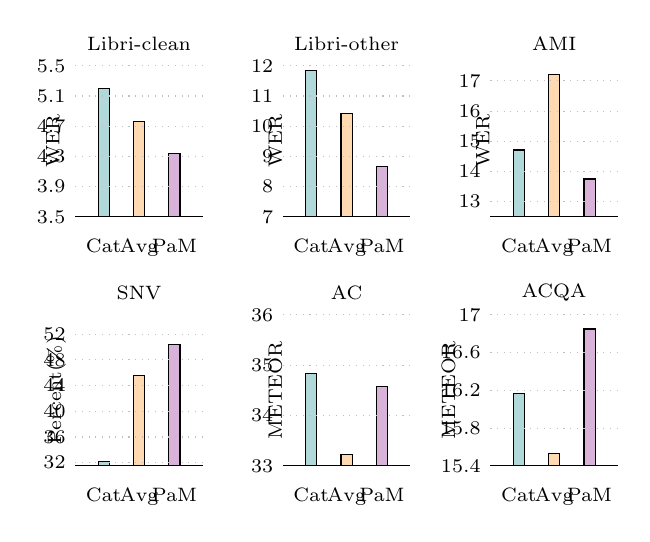
\begin{tikzpicture}

% \def\barbias{2mm}
\def\barbias{0mm}

\begin{scope}[xshift=0em]
\begin{axis}[
at={(0em,0em)},
width=3.2cm, height=3.5cm,
xtick=data,
symbolic x coords={Cat, Avg, PaM},
title={Libri-clean},
title style={anchor=center, font=\scriptsize,yshift=0.2em},
ytick={3.5,3.9,...,5.5},
ylabel={WER},
xlabel style={align=center,font=\scriptsize,xshift=2.2em},
ylabel style={font=\scriptsize,yshift=-1.5em},
x tick style={opacity=0},
y tick style={opacity=0},
x tick label style={anchor=base,font=\scriptsize,yshift=-0.3cm},
y tick label style={font=\scriptsize,/pgf/number format/.cd,fixed,precision=2},
ymajorgrids=true,
y axis line style={opacity=0},
tick align=inside,
axis x line*=bottom,
major grid style={dotted},
axis on top,
enlarge x limits=0.4, 
% legend pos=north east,
% legend style={yshift=4.0em,xshift=0em,legend cell align=left,legend plot pos=right, draw=none, fill=none,legend  columns =-1},
ybar,
bar width=4pt,
ymin=3.5, ymax=5.5]

\addplot[fill=teal!30, bar shift=-\barbias] coordinates {(Cat, 5.2) (Avg, 0) (PaM, 0)};
\addplot[fill=orange!30, bar shift=0mm] coordinates {(Cat, 0) (Avg, 4.76) (PaM, 0)};
\addplot[fill=violet!30, bar shift=\barbias] coordinates {(Cat, 0) (Avg, 0) (PaM, 4.34)};

\end{axis}
\end{scope}

\begin{scope}[xshift=7.5em]
\begin{axis}[
at={(0em,0em)},
width=3.2cm, height=3.5cm,
xtick=data,
symbolic x coords={Cat, Avg, PaM},
title={Libri-other},
title style={anchor=center, font=\scriptsize,yshift=0.2em},
ytick={7,8,...,12},
ylabel={WER},
xlabel style={align=center,font=\scriptsize,xshift=2.2em},
ylabel style={font=\scriptsize,yshift=-1.8em},
x tick style={opacity=0},
y tick style={opacity=0},
x tick label style={anchor=base,font=\scriptsize,yshift=-0.3cm},
y tick label style={font=\scriptsize,/pgf/number format/.cd,fixed,precision=2},
ymajorgrids=true,
y axis line style={opacity=0},
tick align=inside,
axis x line*=bottom,
major grid style={dotted},
axis on top,
enlarge x limits=0.4, 
% legend pos=north east,
% legend style={yshift=4.0em,xshift=0em,legend cell align=left,legend plot pos=right, draw=none, fill=none,legend  columns =-1},
ybar,
bar width=4pt,
ymin=7, ymax=12]

\addplot[fill=teal!30, bar shift=-\barbias] coordinates {(Cat, 11.83) (Avg, 0) (PaM, 0)};
\addplot[fill=orange!30, bar shift=0mm] coordinates {(Cat, 0) (Avg, 10.43) (PaM, 0)};
\addplot[fill=violet!30, bar shift=\barbias] coordinates {(Cat, 0) (Avg, 0) (PaM, 8.68)};

\end{axis}
\end{scope}

\begin{scope}[xshift=15em]
\begin{axis}[
at={(0em,0em)},
width=3.2cm, height=3.5cm,
xtick=data,
symbolic x coords={Cat, Avg, PaM},
title={AMI},
title style={anchor=center, font=\scriptsize,yshift=0.2em},
ytick={12,13,...,17},
ylabel={WER},
xlabel style={align=center,font=\scriptsize,xshift=2.2em},
ylabel style={font=\scriptsize,yshift=-1.8em},
x tick style={opacity=0},
y tick style={opacity=0},
x tick label style={anchor=base,font=\scriptsize,yshift=-0.3cm},
y tick label style={font=\scriptsize,/pgf/number format/.cd,fixed,precision=2},
ymajorgrids=true,
y axis line style={opacity=0},
tick align=inside,
axis x line*=bottom,
major grid style={dotted},
axis on top,
enlarge x limits=0.4, 
% legend pos=north east,
% legend style={yshift=4.0em,xshift=0em,legend cell align=left,legend plot pos=right, draw=none, fill=none,legend  columns =-1},
ybar,
bar width=4pt,
ymin=12.5, ymax=17.5]

\addplot[fill=teal!30, bar shift=-\barbias] coordinates {(Cat, 14.71) (Avg, 0) (PaM, 0)};
\addplot[fill=orange!30, bar shift=0mm] coordinates {(Cat, 0) (Avg, 17.2) (PaM, 0)};
\addplot[fill=violet!30, bar shift=\barbias] coordinates {(Cat, 0) (Avg, 0) (PaM, 13.75)};

\end{axis}
\end{scope}

\begin{scope}[xshift=0em, yshift=-9em]
\begin{axis}[
at={(0em,0em)},
width=3.2cm, height=3.5cm,
xtick=data,
symbolic x coords={Cat, Avg, PaM},
title={SNV},
title style={anchor=center, font=\scriptsize,yshift=0.2em},
ytick={32,36,...,52},
ylabel={Percent(\%)},
xlabel style={align=center,font=\scriptsize,xshift=2.2em},
ylabel style={font=\scriptsize,yshift=-1.5em},
x tick style={opacity=0},
y tick style={opacity=0},
x tick label style={anchor=base,font=\scriptsize,yshift=-0.3cm},
y tick label style={font=\scriptsize,/pgf/number format/.cd,fixed,precision=2},
ymajorgrids=true,
y axis line style={opacity=0},
tick align=inside,
axis x line*=bottom,
major grid style={dotted},
axis on top,
enlarge x limits=0.4, 
% legend pos=north east,
% legend style={yshift=4.0em,xshift=0em,legend cell align=left,legend plot pos=right, draw=none, fill=none,legend  columns =-1},
ybar,
bar width=4pt,
ymin=31.5, ymax=55]

\addplot[fill=teal!30, bar shift=-\barbias] coordinates {(Cat, 32.2) (Avg, 0) (PaM, 0)};
\addplot[fill=orange!30, bar shift=0mm] coordinates {(Cat, 0) (Avg, 45.5) (PaM, 0)};
\addplot[fill=violet!30, bar shift=\barbias] coordinates {(Cat, 0) (Avg, 0) (PaM, 50.4)};

\end{axis}
\end{scope}

\begin{scope}[xshift=7.5em, yshift=-9em]
\begin{axis}[
at={(0em,0em)},
width=3.2cm, height=3.5cm,
xtick=data,
symbolic x coords={Cat, Avg, PaM},
title={AC},
title style={anchor=center, font=\scriptsize,yshift=0.2em},
ytick={33,34,...,36},
ylabel={METEOR},
xlabel style={align=center,font=\scriptsize,xshift=2.2em},
ylabel style={font=\scriptsize,yshift=-1.8em},
x tick style={opacity=0},
y tick style={opacity=0},
x tick label style={anchor=base,font=\scriptsize,yshift=-0.3cm},
y tick label style={font=\scriptsize,/pgf/number format/.cd,fixed,precision=2},
ymajorgrids=true,
y axis line style={opacity=0},
tick align=inside,
axis x line*=bottom,
major grid style={dotted},
axis on top,
enlarge x limits=0.4, 
% legend pos=north east,
% legend style={yshift=4.0em,xshift=0em,legend cell align=left,legend plot pos=right, draw=none, fill=none,legend  columns =-1},
ybar,
bar width=4pt,
ymin=33, ymax=36]

\addplot[fill=teal!30, bar shift=-\barbias] coordinates {(Cat, 34.84) (Avg, 0) (PaM, 0)};
\addplot[fill=orange!30, bar shift=0mm] coordinates {(Cat, 0) (Avg, 33.22) (PaM, 0)};
\addplot[fill=violet!30, bar shift=\barbias] coordinates {(Cat, 0) (Avg, 0) (PaM, 34.58)};

\end{axis}
\end{scope}

\begin{scope}[xshift=15em, yshift=-9em]
\begin{axis}[
at={(0em,0em)},
width=3.2cm, height=3.5cm,
xtick=data,
symbolic x coords={Cat, Avg, PaM},
title={ACQA},
title style={anchor=center, font=\scriptsize,yshift=0.2em},
ytick={15.4,15.8,...,17},
ylabel={METEOR},
xlabel style={align=center,font=\scriptsize,xshift=2.2em},
ylabel style={font=\scriptsize,yshift=-1.2em},
x tick style={opacity=0},
y tick style={opacity=0},
x tick label style={anchor=base,font=\scriptsize,yshift=-0.3cm},
y tick label style={font=\scriptsize,/pgf/number format/.cd,fixed,precision=2},
ymajorgrids=true,
y axis line style={opacity=0},
tick align=inside,
axis x line*=bottom,
major grid style={dotted},
axis on top,
enlarge x limits=0.4, 
% legend pos=north east,
% legend style={yshift=4.0em,xshift=0em,legend cell align=left,legend plot pos=right, draw=none, fill=none,legend  columns =-1},
ybar,
bar width=4pt,
ymin=15.4, ymax=17]

\addplot[fill=teal!30, bar shift=-\barbias] coordinates {(Cat, 16.17) (Avg, 0) (PaM, 0)};
\addplot[fill=orange!30, bar shift=0mm] coordinates {(Cat, 0) (Avg, 15.53) (PaM, 0)};
\addplot[fill=violet!30, bar shift=\barbias] coordinates {(Cat, 0) (Avg, 0) (PaM, 16.85)};

% \legend{Concat, Average, PaM}
\end{axis}
\end{scope}

\end{tikzpicture}











\end{document}


